% Meter dial for the newspaper demo.  xelatex fig-dial.tex
\documentclass{article}
\usepackage[papersize={3.6cm,3.6cm},margin=1mm]{geometry}
\usepackage{tikz}
\pagestyle{empty}
\begin{document}\noindent
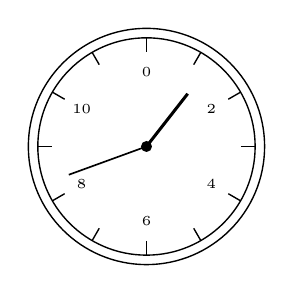
\begin{tikzpicture}[line width=0.5pt]
  \draw (0,0) circle (1.5); \draw (0,0) circle (1.38);
  \foreach \a in {0,30,...,330}{ \draw (\a:1.2) -- (\a:1.38); }
  \foreach \a/\l in {90/0,30/2,330/4,270/6,210/8,150/10}{ \node[font=\tiny] at (\a:0.95) {\l};}
  \draw[line width=1.1pt] (0,0) -- (52:0.85);
  \draw[line width=0.6pt] (0,0) -- (200:1.05);
  \fill (0,0) circle (0.07);
\end{tikzpicture}
\end{document}
